% Created 2023-04-27 Thu 13:54
% Intended LaTeX compiler: pdflatex
\documentclass[11pt]{article}
\usepackage[utf8]{inputenc}
\usepackage[T1]{fontenc}
\usepackage{graphicx}
\usepackage{longtable}
\usepackage{wrapfig}
\usepackage{rotating}
\usepackage[normalem]{ulem}
\usepackage{amsmath}
\usepackage{amssymb}
\usepackage{capt-of}
\usepackage{hyperref}
\author{Yang Huang}
\date{\textit{<2023-04-27 Thu>}}
\title{README}
\hypersetup{
 pdfauthor={Yang Huang},
 pdftitle={README},
 pdfkeywords={},
 pdfsubject={},
 pdfcreator={Emacs 28.2 (Org mode 9.5.5)}, 
 pdflang={English}}
\begin{document}

\maketitle
\tableofcontents


\section{Purpose}
\label{sec:org129e5e0}
To generate a 2D Penrose tiling  from a high-dimension projection
method.

\section{Compilation}
\label{sec:org4e0e7ea}
Type "make".

\section{Usage}
\label{sec:org16455bc}
Type "./test" and then "./viewsites.py"

\begin{center}
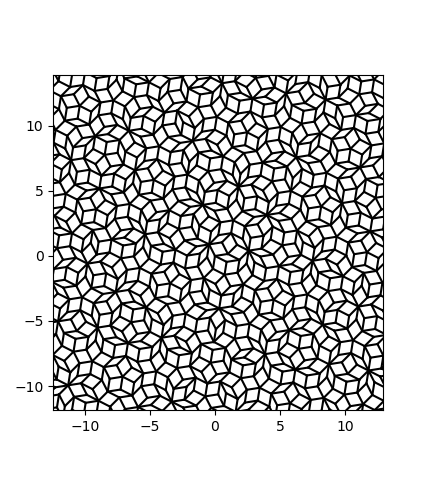
\includegraphics[width=.9\linewidth]{./qcs.png}
\end{center}
\end{document}